% Snowflake Data Engineering — Chapter 15 | original manuscript draft
% Author: Arman Golbidi | Editorial snapshot: 22 October 2026
% Compile: xelatex -interaction=nonstopmode -halt-on-error Snowflake_Data_Engineering_Chapter_15.tex
% Trim: 178 x 254 mm; margins inside 23 mm / outside 17 mm / top-bottom 19 mm.
% Body: 10.75 pt / 13.65 pt leading = 1.27 line-height ratio; code: 8.75 pt.
\documentclass[11pt,twoside]{article}
\usepackage[paperwidth=178mm,paperheight=254mm,inner=23mm,outer=17mm,top=19mm,bottom=19mm,headheight=5mm,headsep=4mm,footskip=9mm]{geometry}
\usepackage{fontspec}
\setmainfont{LibertinusSerif-Regular.otf}[BoldFont=LibertinusSerif-Bold.otf,ItalicFont=LibertinusSerif-Italic.otf,BoldItalicFont=LibertinusSerif-BoldItalic.otf]
\setsansfont{LibertinusSans-Regular.otf}[BoldFont=LibertinusSans-Bold.otf,ItalicFont=LibertinusSans-Italic.otf]
\setmonofont{LibertinusMono-Regular.otf}[Scale=0.91]
\usepackage[english]{babel}
\usepackage{microtype}
\usepackage{setspace}
\setstretch{1.0}
\usepackage{titlesec,enumitem,tabularx,array,booktabs,needspace,fancyhdr,lastpage}
\usepackage[most]{tcolorbox}
\usepackage{tikz}
\usetikzlibrary{arrows.meta,positioning,fit,shapes.misc,calc}
\usepackage{listings}
\usepackage{xcolor}
\usepackage{hyperref}
\usepackage{amsmath}
\hypersetup{colorlinks=true,urlcolor=steelblue,linkcolor=steelblue,pdfauthor={Arman Golbidi},pdftitle={Snowflake Data Engineering - Chapter 15: Capstone: A Production-Ready Energy Data Platform},pdfsubject={English technical book manuscript, fifteenth chapter, 178 x 254 mm}}
\definecolor{navy}{HTML}{15334A}
\definecolor{steelblue}{HTML}{17779B}
\definecolor{teal}{HTML}{12888A}
\definecolor{lightblue}{HTML}{ECF5F7}
\definecolor{papergray}{HTML}{F2F5F6}
\definecolor{inkgray}{HTML}{4A5862}
\definecolor{thinrule}{HTML}{CBD7DB}
\AtBeginDocument{\color{navy}\fontsize{10.75}{13.65}\selectfont}
\setlength{\parindent}{0pt}
\emergencystretch=2.5em
\setlength{\parskip}{3.3pt plus 0.7pt minus 0.6pt}
\setlist[itemize]{leftmargin=4mm,itemsep=1pt,topsep=2pt,parsep=0pt}
\setlist[enumerate]{leftmargin=5mm,itemsep=1pt,topsep=2pt}
\titleformat{\section}{\sffamily\bfseries\color{navy}\fontsize{14}{17}\selectfont}{}{0pt}{}
\titlespacing*{\section}{0pt}{8pt}{4pt}
\titleformat{\subsection}{\sffamily\bfseries\color{steelblue}\fontsize{10.8}{13}\selectfont}{}{0pt}{}
\titlespacing*{\subsection}{0pt}{5pt}{1pt}
\newcommand{\topic}[2]{\subsection*{#1\quad #2}}
\newcommand{\repo}[2]{\par\begingroup\fontsize{8.0}{9.6}\selectfont\sffamily\color{inkgray}\textbf{Project reference:} \href{#2}{#1}. \textit{Not independently executed; rights review pending.}\par\endgroup}
\newtcolorbox{insight}[1][]{enhanced,breakable,colback=lightblue,colframe=thinrule,boxrule=.45pt,arc=1.3mm,left=2.8mm,right=2.8mm,top=1.8mm,bottom=1.8mm,before skip=5pt,after skip=5pt,#1}
\newtcolorbox{whitebox}[1][]{enhanced,breakable,colback=papergray,colframe=thinrule,boxrule=.35pt,arc=1mm,left=2.6mm,right=2.6mm,top=1.5mm,bottom=1.5mm,before skip=4pt,after skip=5pt,#1}
\lstdefinestyle{chaptercode}{basicstyle=\ttfamily\fontsize{8.75}{10.7}\selectfont,backgroundcolor=\color{papergray},frame=single,framerule=.35pt,rulecolor=\color{thinrule},breaklines=true,columns=fullflexible,keepspaces=true,showstringspaces=false,aboveskip=5pt,belowskip=5pt,xleftmargin=2mm,xrightmargin=1mm,framexleftmargin=2mm,framexrightmargin=1mm}
\lstset{style=chaptercode}
\pagestyle{fancy}
\fancyhf{}
\fancyhead[LE]{\sffamily\fontsize{7.6}{9}\selectfont\color{inkgray}\textsc{Snowflake Data Engineering}}
\fancyhead[RO]{\sffamily\fontsize{7.6}{9}\selectfont\color{inkgray}\textsc{15 / Energy Capstone}}
\fancyfoot[LE,RO]{\sffamily\bfseries\fontsize{8.2}{9}\selectfont\color{steelblue}\thepage}
\fancyfoot[LO,RE]{\sffamily\fontsize{7.6}{9}\selectfont\color{inkgray}Arman Golbidi \quad | \quad Chapter 15}
\renewcommand{\headrulewidth}{0.35pt}
\renewcommand{\footrulewidth}{0pt}
\setcounter{page}{265}
\raggedbottom

\begin{document}
% Page 265 -- chapter opening
{\sffamily\bfseries\fontsize{9}{11}\selectfont\color{steelblue} CHAPTER 15 \hfill INTEGRATE / VERIFY / OPERATE}\par\vspace{3mm}
{\sffamily\bfseries\fontsize{19}{22}\selectfont\color{navy} Capstone: A Production-Ready\\Energy Data Platform}\par\vspace{2mm}
{\sffamily\fontsize{11}{14}\selectfont\color{steelblue} Can another engineer rebuild, verify and operate the whole system?}\par\vspace{3mm}
\begin{insight}\textbf{The dashboard is not the deliverable.} Imagine a Finnish energy analyst opening a clear Power BI report at 08:00. A wind-generation number is wrong. Did the source publish a correction? Did yesterday's batch run twice? Was an invalid row quietly accepted? Or did the report refresh before the silver table? Without a traceable answer, the pleasant dashboard is an operational liability.\end{insight}
This final chapter turns the concepts developed across Chapters~1--14 into one governed engineering product: the \emph{Finland Energy Analytics} capstone. The aim is a system that can be inspected, rerun, tested and handed over. The printed walkthrough provides architecture, acceptance criteria, selected implementation patterns and evidence. The companion project contains longer scripts, fixtures, validation, decision records and incident procedures.
\begin{whitebox}\textbf{What you will deliver}\par
A documented ingestion and transformation chain from immutable synthetic source events to bronze, silver and gold; versioned contracts and reproducible checks; role and cost policies; a BI semantic contract; a monitoring and recovery runbook; and a release review that distinguishes proved offline behaviour from Snowflake features still requiring live integration tests.\end{whitebox}
\textbf{Prerequisites.} Chapters~1--14 and elementary SQL/Python. No Snowflake credits are needed for the \emph{offline acceptance fixture}; a real deployment requires a test account, controlled role grants, an approved spend limit and a designated owner. All sample energy readings in this chapter are synthetic; no production Finnish electricity data has been downloaded into the book package.
\begin{center}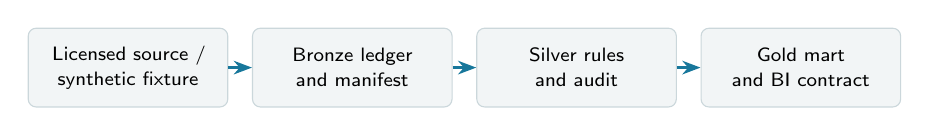
\begin{tikzpicture}[>=Stealth,every node/.style={font=\sffamily\fontsize{7.3}{9}\selectfont},n/.style={draw=thinrule,rounded corners=1mm,fill=papergray,align=center,text width=23mm,minimum height=10mm}]
\node[n](a){Licensed source /\\synthetic fixture};\node[n,right=3mm of a](b){Bronze ledger\\and manifest};\node[n,right=3mm of b](c){Silver rules\\and audit};\node[n,right=3mm of c](d){Gold mart\\and BI contract};
\draw[->,thick,steelblue](a)--(b);\draw[->,thick,steelblue](b)--(c);\draw[->,thick,steelblue](c)--(d);
\end{tikzpicture}\\{\fontsize{8}{9}\selectfont\color{inkgray}Figure 15.1. Every arrow needs a contract, observable evidence and a recovery path.}\end{center}
\textbf{Release principle.} ``Production-ready'' describes the engineered safeguards and documented gates, not a claim that this teaching package has passed a live Snowflake security review or been deployed to the Finnish grid.

\newpage

% Page 266 -- 15.1 part 1
\section*{15.1\quad Business scenario, assumptions, and acceptance criteria}
\topic{15.1.1}{Business scenario and stakeholder decisions}
The business sponsor needs one trusted view of renewable and other generation readings at an agreed time grain. The operations analyst wants to know whether an observed change is a real generation movement or a corrected source delivery. A data steward wants evidence of origin and licence. A platform operator needs to diagnose missing data without guessing which job to restart. These are different decisions, so a single dashboard acceptance test cannot represent all of them.
\begin{center}\small\begin{tabularx}{\linewidth}{@{}p{27mm}X X@{}}\toprule
Stakeholder & Decision & Required evidence\\\midrule
Energy analyst & Compare generation categories & UTC grain, unit and version\\
Data steward & Permit publication & Licence and source lineage\\
Operator & Recover a failed ingest & File checksum and run ledger\\
Platform owner & Approve release & Tests, grants and spend review\\\bottomrule
\end{tabularx}\end{center}
In the educational scenario, a source provider may publish a revised wind value for an existing UTC interval. The platform must retain the earlier evidence, select the valid newer revision, and publish a single current observation. A deliberate duplicate delivery must not double the energy KPI. A logical deletion is not equivalent to an energy reading of zero: deletion changes which key is visible; zero is a legitimate measurement where the source contract permits it.
\topic{15.1.2}{Dataset assumptions and limitations}
The companion fixture has twelve \emph{synthetic} delivered rows, including a duplicate event, one superseded version, a logical deletion and two invalid records. Its final accepted view contains six readings totalling \textbf{66.000 MWh}. The source label \texttt{DEMO\_GRID} is invented. The timestamp is in UTC; generation categories are invented teaching values, not estimates of Finnish production. These six rows cannot support a credible national trend, a machine-learning forecast or an operational energy decision.
\begin{insight}\textbf{Assumption register.} Define the natural key as \emph{provider + technology + interval\_utc}; define \texttt{REVISION} as a positive, monotonically increasing integer for each key. Accept only \texttt{UPSERT} or \texttt{DELETE}; require nonnegative finite MWh; require DELETE to carry zero; and reject conflicting payloads at an equal key and revision. Each rule is intentionally testable.\end{insight}
\textbf{Failure to avoid.} A business sponsor signs off on a attractive chart without noticing that a wind revision is counted twice. The correct first acceptance meeting examines a six-row gold export, a rejected-row log and a small set of named invariants.

\newpage

% Page 267 -- 15.1 part 2
\topic{15.1.3}{Explicit acceptance and review criteria}
Define acceptance before implementation. A successful pipeline is not merely one that returns rows; it demonstrates functional correctness, privacy of access, recoverability, repeatability and an economically bounded operating path. A reproducible trial records the input hash, code revision, run commands, timestamp, failed checks and operator identity. The acceptance document should name who is authorised to waive a check; the default for a broken invariant is \textbf{do not publish}.
\begin{center}\small\begin{tabularx}{\linewidth}{@{}p{11mm}p{36mm}X@{}}\toprule
ID & Release criterion & Evidence artifact\\\midrule
A01 & Exactly six current rows & Gold CSV and uniqueness test\\
A02 & Total equals 66.000 MWh & Independent Python oracle\\
A03 & Two rows quarantined & Row-level reasons and count\\
A04 & Replay leaves result unchanged & Double-run comparison\\
A05 & Access policy reviewed & Negative permission test plan\\
A06 & Recovery and cost defined & Runbook, budget and rollback\\\bottomrule
\end{tabularx}\end{center}
The first four checks can be demonstrated offline with the shipped fixture. A05 and the Snowflake part of A06 cannot be declared successful by a local Python test. The release record therefore has two dimensions: \emph{offline demonstration passed} and \emph{cloud deployment not yet approved}. This distinction prevents a common portfolio mistake: reporting an architectural design as if production controls were already operating.
A useful acceptance matrix has three columns for every criterion: the observable result, the evidence path and the responsible reviewer. For example, an idempotent replay check must compare \emph{business results and audit state}, not merely show that SQL completed without an exception. An apparently identical final sum could hide two duplicated wind rows and two missing solar rows; include key-level comparisons and row counts.
\begin{whitebox}\textbf{Decision record 15-01: proof before deployment.} The capstone uses the offline fixture as a deterministic correctness oracle and treats Snowflake integration, Power BI report operation, hosted event notifications and external AI as separately gated extensions. \textbf{Reason:} local reproducibility must not depend on account permissions or variable credit charges. \textbf{Cost:} the offline run cannot reveal warehouse performance or actual account privileges.\end{whitebox}
\repo{P006: Northstar data engineering; P176: telecom operations analytics}{https://github.com/Snowflake-Labs/sfguide-snowflake-northstar-data-engineering}
\textbf{Learning check.} Which two accepted results would you inspect to prove that the same input file produced the same publishable facts after replay? Include a business-key comparison, not only a checksum of the source.

\newpage

% Page 268 -- 15.2 part 1
\section*{15.2\quad Source selection, architecture, and data contracts}
\topic{15.2.1}{Fingrid and Statistics Finland source options}
The starting point for an actual Finnish energy product is a \emph{source catalogue}, not a web scraper. Fingrid's open-data portal publishes datasets relevant to Finland's electricity system; Statistics Finland offers statistical datasets and machine-readable services. They serve different grains and meanings. A Fingrid series might describe power or energy at operational intervals; a Statistics Finland table might describe regional, monthly or annual statistical aggregates. Do not join these blindly on a date and call the result ``hourly generation.''
For each candidate, record dataset title and identifier, publisher, definition, measurement unit, spatial coverage, update policy, timestamp semantics, historical revisions, rate limits, reuse terms and the exact time of collection. A source may express power in MW, while an accepted observation fact uses energy in MWh. Conversion requires an interval duration and an explicit integration rule; multiplying a power reading by ``one hour'' without verifying its sampling semantics is an invented measurement.
\begin{center}\small\begin{tabularx}{\linewidth}{@{}p{28mm}X X@{}}\toprule
Question & Fingrid-type feed & Statistics Finland-type table\\\midrule
Likely grain & Operational series; varies by dataset & Published statistical periods\\
Primary check & Timestamp/unit revision & Definitions, classifications, vintages\\
Collection & API or published export & PX-Web/structured download\\
Caution & MW is not automatically MWh & National totals are not event rows\\\bottomrule\end{tabularx}\end{center}
The teaching package does not include a live fetcher or redistribute an external dataset. That avoids an implicit claim that any one Fingrid endpoint, key policy or licence will stay unchanged. The next real-data milestone would select one precise dataset, snapshot its metadata and run a limited authorised retrieval; it should be reviewed as a separate deliverable.\par\begingroup\fontsize{8}{9.5}\selectfont\color{inkgray}Source portals: \href{https://data.fingrid.fi/en/}{Fingrid Open Data}; \href{https://stat.fi/en/services/statistical-data-services/open-data-and-interfaces}{Statistics Finland open data}.\par\endgroup
\begin{insight}\textbf{Source checkpoint.} A credible lineage row is \emph{publisher + dataset ID + source URL + access time + version or ETag/hash + licence snapshot}. A convenient public URL is not proof of continuous access or commercial redistribution rights for every asset on the portal.\end{insight}

\newpage

% Page 269 -- 15.2 part 2
\topic{15.2.2}{Dataset licensing, snapshots, and provenance}
A dataset is useful only if a reviewer can say which version produced an answer. Store the original bytes, compute SHA-256 and keep the publisher metadata separately. An API response might change without a filename changing; an immutable snapshot plus request metadata makes investigations possible even after the upstream resource has been revised. If the provider forbids redistribution, keep the raw data in authorised storage and ship only independently authored synthetic fixtures with the book.
Statistics Finland describes its open statistical data as available under Creative Commons Attribution 4.0 with source attribution; the project still must check each dataset and any exceptions at acquisition time. For Fingrid, inspect the terms attached to the exact dataset and API rather than transferring a generic licence assumption from another portal. This publication is independent of both institutions and is not an endorsed Finnish energy service.
The manifest should record \texttt{sha256}, \texttt{original\_name}, \texttt{retrieved\_at\_utc}, \texttt{publisher}, \texttt{dataset\_id}, \texttt{licence\_url}, \texttt{schema\_version} and \texttt{row\_count}. Use checksums to detect altered input bytes, not to prove truthfulness of a measurement. Source accuracy requires separate domain validation and, where justified, cross-provider reconciliation.
\begin{lstlisting}[language=Python]
# Pure local provenance check; no cloud call.
from hashlib import sha256
from pathlib import Path
p = Path('project/data/energy_revisions.csv')
digest = sha256(p.read_bytes()).hexdigest()
assert len(digest) == 64
print('fixture sha256:', digest)
\end{lstlisting}
A timestamp is also part of provenance. Record both \emph{event time} (when the measurement applies) and \emph{processing time} (when the pipeline received or validated it). When a correction arrives late, event-time aggregation remains stable while ingest-time audit reflects the revision. That separation is essential for reconstructing what a user could have known at a past reporting cutoff.
\begin{whitebox}\textbf{Rights and source ledger.} The companion \texttt{references/source\_register.md} identifies external portals as optional research options, not as executed inputs. It labels every delivered reading as synthetic, so a redistribution audit can distinguish source citations from actual data assets.\end{whitebox}

\newpage

% Page 270 -- 15.2 part 3
\topic{15.2.3}{Architecture and versioned data contracts}
The reference design separates immutable evidence from mutable interpretation. Ingestion writes the bronze event ledger. Silver enforces schema and business rules, resolves versions and quarantines failures. Gold publishes an intentionally narrow metric contract. A separate access boundary exposes reporting views to Power BI rather than handing the BI role permission to query raw event payloads.
\begin{center}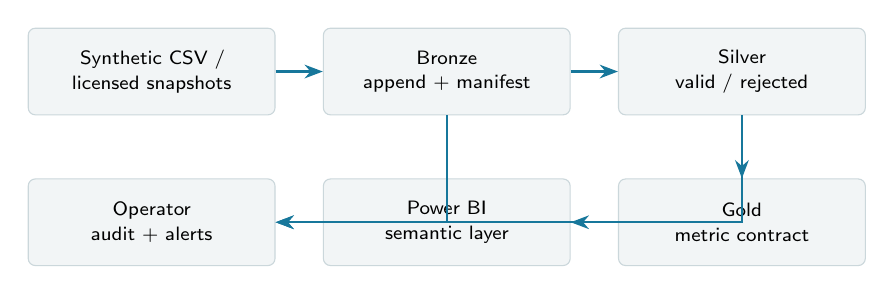
\begin{tikzpicture}[>=Stealth,every node/.style={font=\sffamily\fontsize{7.1}{8.8}\selectfont},n/.style={draw=thinrule,rounded corners=.9mm,fill=papergray,align=center,text width=29mm,minimum height=11mm}]
\node[n](a){Synthetic CSV /\\licensed snapshots};\node[n,right=6mm of a](b){Bronze\\append + manifest};\node[n,right=6mm of b](c){Silver\\valid / rejected};
\node[n,below=8mm of c](d){Gold\\metric contract};\node[n,left=6mm of d](e){Power BI\\semantic layer};\node[n,left=6mm of e](f){Operator\\audit + alerts};
\draw[->,thick,steelblue](a)--(b);\draw[->,thick,steelblue](b)--(c);\draw[->,thick,steelblue](c)--(d);\draw[->,thick,steelblue](d)--(e);\draw[->,thick,steelblue](b)|-(f);\draw[->,thick,steelblue](c)|-(f);
\end{tikzpicture}\\{\fontsize{8}{9}\selectfont\color{inkgray}Figure 15.2. Audit and consumption are separate access paths.}\end{center}
The \texttt{energy-event/v1} contract has seven required fields: event ID, provider, technology, UTC timestamp, positive revision, decimal MWh and \texttt{UPSERT}/\texttt{DELETE} operation. A later version may add an optional quality code; it must not silently reinterpret historical MWh as kWh. Changing units or natural-key meaning is a breaking change and deserves a new schema version with an explicit migration plan.
\begin{whitebox}\textbf{Contract review questions.} What is the business key? Can two events disagree at the same revision? Is a missing hour an error, or a source that did not promise hourly completeness? What identifies a deleted observation? Which columns are sensitive, and what role may see them? Each answer belongs in the contract, not in a dashboard footnote.\end{whitebox}
\repo{P011: green-energy IoT example; P169: predictive maintenance}{https://github.com/nbaubek/green-energy-iot-de-project}
\textbf{Failure mode.} Treating the CSV's delivery order as the truth causes an older Hydro event to replace a newer one after replay. Sort by business revision, and fail the release on an ambiguous same-revision conflict.

\newpage

% Page 271 -- 15.3 part 1
\section*{15.3\quad Reproducible environment and repository structure}
\topic{15.3.1}{Environment automation and roles}
A reproducible environment has more than a diagram of objects. It specifies a version-controlled deployment order, who can create objects and which tests run without cloud access. The least-privileged application role should not create account-wide grants, policies or integrations. One-time administrator-approved bootstrap is distinct from repeatable engineering deployment. Production and development objects must not share an unqualified schema name or a write-enabled service identity.
Create a dedicated database or sandbox namespace only after the account owner approves the plan. Use a small, auto-suspending warehouse for test SQL, record its name in environment configuration and prohibit accidental escalation to a large size. Resource monitors can govern certain warehouse consumption, but do not promise they cap every serverless or AI charge. Avoid provisioning a continuously refreshing object merely to demonstrate one reading update.
\begin{lstlisting}[language=SQL]
-- Cloud example: run ONLY in an approved sandbox.
USE ROLE <APPROVED_DEPLOY_ROLE>;
USE WAREHOUSE <APPROVED_SMALL_WAREHOUSE>;
CREATE SCHEMA IF NOT EXISTS ENERGY_LAB.BRONZE;
CREATE SCHEMA IF NOT EXISTS ENERGY_LAB.SILVER;
CREATE SCHEMA IF NOT EXISTS ENERGY_LAB.GOLD;
\end{lstlisting}
\textbf{Important:} placeholder role and warehouse names are not executable Snowflake identifiers. Replace them from an approved environment file, verify privileges and record the grants separately. Database creation and role management are \emph{not} auto-run by the companion project.
\topic{15.3.2}{Folder structure and immutable dependencies}
The repository root contains \texttt{project/}, \texttt{operations/}, an ADR folder and a test-evidence folder. The project holds a fixture, a Python acceptance oracle, SQL examples, contracts, BI definitions and CI notes. A future deployed release should include a lockfile or immutable container digest; a vague request to install the latest packages makes yesterday's run irreproducible. Avoid embedding passwords in config files or example commands.
\begin{insight}\textbf{Two execution tiers.} Tier~1 runs offline on Python's standard library and enforces data invariants. Tier~2 runs only after cloud approval: create scoped objects, stage bytes, load, compare the gold view and perform negative grants tests. Success in Tier~1 is necessary, but not sufficient, for a production deployment.\end{insight}

\newpage

% Page 272 -- 15.3 part 2
\topic{15.3.3}{Test fixtures and cleanup procedures}
A good fixture represents the failures the system promises to tolerate. Our twelve deliveries contain an identical repeated event, a revised Wind observation, an old Hydro version, a tombstone for a \texttt{TEST} category and invalid source values. Rather than treating the fixture as disposable random data, record its SHA-256 hash in the acceptance output. Re-running the same code against the same file must give the same six visible business keys and total.
A negative test should be reversible. For example, corrupt a copy of the file to change a field name, run the schema-contract assertion and confirm a hard failure. Another test can insert two different payloads for the same natural key and revision; this must block publication rather than elect an arbitrary winner. No test should need to alter the original fixture.
\begin{center}\small\begin{tabularx}{\linewidth}{@{}p{33mm}X@{}}\toprule
Fixture variant & Expected behaviour\\\midrule
Repeated identical event & Deduplicate; no extra energy\\
Valid higher revision & Select newer reading at same key\\
Revision zero & Quarantine under v1 contract\\
Negative MWh & Quarantine with reason\\
Equal-revision conflict & Stop release and investigate\\
Zero-valued DELETE & Remove key from current view\\\bottomrule\end{tabularx}\end{center}
Cleanup is also part of reproducibility. Do not place an unconditional \texttt{DROP DATABASE} inside a reader lab. Instead, use a clearly named sandbox deployment, enumerate the exact objects the exercise created, retain evidence outside that sandbox, and require an authorised person to uncomment destructive SQL. Confirm that no production references or shared stages depend on the objects before removal.
\begin{whitebox}\textbf{Rebuild proof.} A reviewer should clone the archive, run \texttt{python -m unittest discover -s project/tests -v}, execute the offline oracle, and compare its structured output with the acceptance contract. If an assertion fails, the review stops; the engineer diagnoses the change and supplies a new fixture version and release note rather than weakening the test.\end{whitebox}
\repo{P120: Snowflake DevOps data projects}{https://github.com/Snowflake-Labs/sfguide-getting-started-with-devops-data-projects-in-snowflake}
\textbf{Check.} Why is testing the cleanup path not equivalent to adding \texttt{DROP SCHEMA CASCADE} to an automated pipeline? Write a rollback plan that protects evidence and does not exceed the role's authority.

\newpage

% Page 273 -- 15.4
\section*{15.4\quad Batch and continuous ingestion design}
\topic{15.4.1}{Reliable batch ingestion}
For the baseline, batch ingestion wins on simplicity. Freeze the input, sign a manifest, load the raw rows, retain filename and row number, then validate each typed field in silver. A batch boundary provides a natural replay unit and makes a postmortem easier: an operator can identify exactly which archived input produced a broken run. A unique event ID is useful metadata, but the \emph{business} identity still consists of provider, technology and interval.
\begin{lstlisting}[language=SQL]
-- Simplified source audit: inspect after COPY, not before.
SELECT source_file, COUNT(*) AS delivered_rows
FROM ENERGY_LAB.BRONZE.EVENT_LEDGER
GROUP BY source_file ORDER BY source_file;
\end{lstlisting}
Store the SHA-256 digest in an independent manifest; source metadata alone does not prove file integrity. Snowflake's \texttt{COPY INTO} maintains load history, but file-level deduplication and load metadata are not substitutes for correction semantics at the business-key level. A \texttt{FORCE} reload, accidental file rename or a different ingestion route can duplicate deliveries. The silver contract must survive those conditions.
\topic{15.4.2}{Optional continuous ingestion}
An event-driven variant may use Snowpipe for staged-file notifications or a streaming connector for row-level delivery. Select it only when measured freshness needs justify a harder operational model. Decide how offsets, acknowledgements, schema changes and dead-letter queues work before advertising ``exactly once.'' Source acknowledgements cannot prevent all application-level replays; deduplicate downstream with stable identities and revision rules.
\topic{15.4.3}{Audit metadata and replay checks}
A load ledger records run ID, source snapshot hash, ingest start and end, observed row count, quarantine count, publish outcome and operator. On retry, reconcile both source and target counts, and compare gold business-key sets. A successful \texttt{COPY} does not certify valid business values or dashboard consistency.
\begin{insight}\textbf{Correctness gate.} Replay the twelve-row synthetic fixture twice. The second pass may produce another processing log, but it must not produce a seventh gold observation or change 66.000 MWh. Treat increased processing cost as a separate operational concern.\end{insight}
\repo{P073: Kafka streaming reference; P177: IoT pipeline}{https://github.com/Snowflake-Labs/sfguide-kafka-interactive-tables-streaming}

\newpage

% Page 274 -- 15.5 part 1
\section*{15.5\quad Bronze-to-silver data quality and transformations}
\topic{15.5.1}{Raw bronze lineage}
Bronze should preserve evidence, not attempt to repair the past. Retain the original delivery order, literal values, operation and revision even when a value is malformed. Add only audit columns such as ingestion timestamp, source file, source row number and a stable run identifier. A negative value must remain visible to the quarantine investigation rather than disappear inside an ``ignore bad records'' option.
\begin{lstlisting}[language=SQL]
CREATE TABLE IF NOT EXISTS ENERGY_LAB.BRONZE.EVENT_LEDGER (
  event_id VARCHAR, provider VARCHAR,
  technology VARCHAR, interval_utc VARCHAR,
  revision_raw VARCHAR, energy_raw VARCHAR,
  operation VARCHAR, source_file VARCHAR,
  source_row NUMBER, loaded_at TIMESTAMP_LTZ
);
\end{lstlisting}
The sample SQL uses raw strings for uncertain fields so the platform can retain an invalid revision or quantity without aborting the entire file. In a live account, configure the file format and stage independently, test row parsing with a tiny file, and inspect whether the chosen error mode matches the capture obligation. Keep the complete audit trail only as long as the approved retention policy permits.
A commonly tempting shortcut is to trust an automatically inferred schema and cast every field during \texttt{COPY}. That may be acceptable for a controlled internal feed, but it can destroy the particular malformed value an analyst needs to diagnose. Bronze and silver have different jobs: one captures what arrived; the other declares what the business accepts.
\begin{whitebox}\textbf{Lineage invariant.} For every accepted silver observation, a reviewer must be able to locate its source event and input snapshot. Conversely, every delivered source row has a documented disposition: selected, superseded, exact duplicate, logically deleted or rejected. No row should vanish without classification.\end{whitebox}
\textbf{Learning check.} A source sends wind 12.000 MWh, then wind 14.000 MWh for the same interval. Which bronze rows remain? Which silver value is current? What evidence is necessary to show that the first row was deliberately superseded rather than lost?

\newpage

% Page 275 -- 15.5 part 2
\topic{15.5.2}{Silver standardisation and DST handling}
The acceptance contract requires an ISO-8601 UTC timestamp with a trailing \texttt{Z}. This deliberately avoids ambiguous local times during Finland's daylight-saving transitions. A time like \texttt{03:30} on a local clock may be nonexistent during spring transition or occur twice during autumn transition. Never infer the offset from a naive timestamp using a fixed ``Finland is UTC+2'' rule. Instead, preserve the source timezone identifier and offset, normalise to UTC, and retain a separate display dimension for \texttt{Europe/Helsinki}.
For the synthetic fixture, \texttt{2026-03-01T10:00:00Z} is already UTC. The test suite verifies a canonical structure, positive revision, declared operation and decimal quantity. The source contract defines what happens if timestamps include milliseconds or offsets: either version the contract and parse them explicitly, or quarantine them. A permissive parser that silently changes interpretation creates a false sense of completeness.
\begin{lstlisting}[language=SQL]
-- Inspect validation results before publishing.
SELECT event_id, technology, energy_raw,
       TRY_TO_DECIMAL(energy_raw,18,3) AS energy_mwh,
       TRY_TO_NUMBER(revision_raw) AS revision
FROM ENERGY_LAB.BRONZE.EVENT_LEDGER;
\end{lstlisting}
Casting with \texttt{TRY\_TO\_DECIMAL} allows the query to expose unparseable values as NULL. However, it must be paired with an explicit \emph{error classification}: NULL, nonfinite/invalid input and legitimate zero are not interchangeable. A valid deletion carries zero MWh but changes current-row visibility. A valid zero production reading remains an \texttt{UPSERT}.
\begin{insight}\textbf{A dangerous shortcut.} Grouping by \texttt{TO\_DATE(interval\_utc)} before establishing the intended timezone can shift observations across local reporting dates. Publish an explicit UTC reporting grain; local calendar presentation belongs in a named, tested conversion layer.\end{insight}
The final model uses consistent decimal arithmetic, not floating-point sums, for deterministic demonstration totals. Real source precision may differ by dataset and must be recorded with units and acceptable rounding rules.

\newpage

% Page 276 -- 15.5 part 3
\topic{15.5.3}{Completeness, uniqueness, and range tests}
Data quality is a contract with failure categories. First verify schema shape and parseable typed values. Next apply domain conditions: revision greater than zero, operation in the approved list, MWh nonnegative and deletion quantity equal to zero. Finally apply stateful consistency rules: unique current business key and no conflicting payloads at the same revision. Detect exact duplicate deliveries without treating them as evidence of additional electricity.
The table below separates \emph{fixture} assertions from \emph{real-world} expectations. Because the fixture contains six categories at one interval, its final row count is six. A real feed cannot be assumed to provide exactly six categories or a new row every hour unless the provider's contract makes that guarantee.
\begin{center}\small\begin{tabularx}{\linewidth}{@{}p{27mm}X X@{}}\toprule
Control & Synthetic fixture expectation & Production interpretation\\\midrule
Uniqueness & Six distinct current keys & Unique at agreed fact grain\\
Validity & Two rejected deliveries & Quarantine rate threshold\\
Energy range & No negative MWh & Domain and unit policy\\
Timeliness & Fixed UTC interval & Source SLA and observed lag\\
Revisions & Wind rev. 2 wins & Deterministic version ordering\\\bottomrule\end{tabularx}\end{center}
Test both positive and negative behaviour. The companion unit suite injects header drift and a same-revision conflict and expects hard failures. An acceptance suite that only checks successful records is dangerously incomplete: it cannot prove that a malformed event would be stopped before reaching a report.
\begin{whitebox}\textbf{Quality disposition ledger.} The offline oracle records twelve delivered rows; one exact repeated delivery; two rejected rows; one tombstoned business key; six visible rows; and 66.000 MWh. These categories describe different stages of a stateful projection and are not additive in one simple row-count equation. Use the event-level disposition ledger to reconcile each record exactly once.\end{whitebox}
\repo{P178: medallion case; P179: bronze-silver-gold pipeline}{https://github.com/dabbiruavinash/Snowflake-E-Commerce-Medallion-Architecture-Project}
\textbf{Check.} Explain why a successful type cast does not guarantee a correct business key, and why a null count alone cannot validate the impact of a logical deletion.

\newpage

% Page 277 -- 15.6
\section*{15.6\quad Gold marts, KPIs, and incremental refreshes}
\topic{15.6.1}{Gold star schema and published KPIs}
Gold is a product contract rather than a dumping ground for every source column. Define \texttt{fct\_energy\_hourly} at one row per provider, technology and UTC interval, with an MWh measure and a selected revision. A technology dimension contains controlled labels; a calendar dimension makes UTC and agreed local-display attributes explicit. If there is only one source provider in the demonstration, do not pretend that the fact supports nationwide reconciliation.
\begin{lstlisting}[language=SQL]
-- Demonstration acceptance query after the silver view.
SELECT COUNT(*) AS visible_rows,
       SUM(energy_mwh) AS total_mwh
FROM ENERGY_LAB.GOLD.FCT_ENERGY_HOURLY;
-- Expected for the shipped fixture: 6 and 66.000.
\end{lstlisting}
\topic{15.6.2}{Incremental refresh correctness}
An incremental pipeline must preserve a key's \emph{latest approved state}, including a tombstone, not merely append each newly received \texttt{UPSERT}. Reprocessing a batch can change history when corrections arrive, so the incremental predicate must include a revision or processing-watermark strategy and a repair window for late events. Prefer a deterministic \texttt{MERGE} source with exactly one row per target business key. When multiple source rows match a target, many MERGE designs become nondeterministic or error-prone.
For a Dynamic Table alternative, select and test a supported refresh mode and monitor actual lag; \texttt{TARGET\_LAG} is a freshness goal, not a guaranteed refresh interval. A dbt incremental model is another option, but its unique key and delete strategy must be explicit. The reference architecture documents one chosen method per deployment rather than mixing three orchestration mechanisms for the same gold table.
\topic{15.6.3}{Stakeholder acceptance checks}
The BI owner's sign-off should compare exact key-level results, not only totals. Require the expected Wind revision 2 value of 14.000 MWh, no visible \texttt{TEST} tombstone key, six distinct rows and the accepted total. Also show a metric-definition sheet: whether \emph{net position} includes consumption, whether an MWh sum covers a full reporting period, and what a missing observation means. In this capstone, consumption is not in the base six-row source; any consumption KPI is a separate, explicitly synthetic extension.
\begin{insight}\textbf{Gold promise.} The same filtered fact table and metric definition must serve the SQL check, the Python oracle and the BI measure. A dashboard must not have a separate, undocumented rounding or duplicate-resolution rule.\end{insight}
\repo{P039: Snowflake dbt medallion example}{https://github.com/Jb-Analytics/snowflake-dbt-tpch-medallion}

\newpage

% Page 278 -- 15.7
\section*{15.7\quad Python components, tests, and CI/CD}
\topic{15.7.1}{Reusable Python components}
Separate parsing, validation, revision resolution, publication and the release gate. The supplied \texttt{project/python/capstone.py} exposes these steps as importable functions and uses Python's standard library to minimise external dependencies. It is an \emph{offline acceptance oracle}, not a substitute Snowpark runtime or a connector to real Fingrid measurements. This small boundary permits a reviewer to establish the intended behaviour before validating equivalent SQL against a Snowflake test schema.
\begin{lstlisting}[language=Python]
from pathlib import Path
from capstone import evaluate, release_gate
rows, rejected, audit = evaluate(
    Path('project/data/energy_revisions.csv'))
assert release_gate(rows, rejected, audit)['status'] == 'ACCEPT'
assert audit['visible_rows'] == 6
assert audit['total_mwh'] == '66.000'
\end{lstlisting}
\topic{15.7.2}{Unit and integration test matrix}
Unit tests prove the local code rejects schema drift, invalid decimals, negative values, duplicate deliveries, forbidden operations and conflicting revisions. Integration tests must separately prove the cloud SQL yields the same expected rows, that scoped roles cannot read raw protected data, and that the BI dataset can refresh after a verified publish. Query correctness can be tested offline; network policy, billing effects and grants cannot.
\begin{center}\small\begin{tabularx}{\linewidth}{@{}p{30mm}X X@{}}\toprule
Test tier & Evidence & Release state\\\midrule
Python offline & Actual unittest result & Executed in package\\
Snowflake SQL & Query ID and assertion output & Pending approved account\\
Power BI & Refresh log, screenshots & Pending Desktop/service\\
Security/cost & Negative access and meter & Pending administrator review\\\bottomrule\end{tabularx}\end{center}
\topic{15.7.3}{CI/CD safety and release tags}
The CI example runs offline tests on an isolated runner without credentials. It must not deploy the cloud schema from a public pull request. A separately reviewed deployment job should use short-lived credentials from a managed secret store, verify the target account and environment, require an approval step and emit immutable release metadata. Name a tag such as \texttt{ch15-capstone-review-v1}; the archive does not falsely claim that a public tag already exists.
\repo{P108: Airflow and Snowflake integration example}{https://github.com/astronomer/etl-elt-airflow-snowflake}
\textbf{Check.} Why can a successful GitHub Actions job still be insufficient evidence that a role cannot select from a sensitive Snowflake table?

\newpage

% Page 279 -- 15.8
\section*{15.8\quad Power BI dashboards and optional AI extension}
\topic{15.8.1}{BI semantic model and dashboards}
The report contract should expose the approved gold view with a clearly declared UTC time grain and a sum of MWh. Use a star schema with single-direction dimension-to-fact relationships where practicable. Measures should compute at the model's filter context; they must not silently aggregate a second, incompatible grain. A summary page can show total generation, generation by technology, time-series trend and a source-freshness indicator. An audit page should display the dataset version and last completed refresh, not a fabricated ``real-time'' badge.
\begin{lstlisting}
-- DAX measure for a table of additive MWh facts.
Generation MWh :=
    SUM ( 'fct_energy_hourly'[energy_mwh] )
\end{lstlisting}
Power BI Import can simplify interactive reads but adds a dataset-refresh boundary; DirectQuery asks Snowflake for data during interactions and can amplify warehouse work. Choose based on volume, concurrency, required freshness and measured response time rather than assuming one is universally faster. Review the current connector, identity, privacy level and gateway or cloud-authentication requirements before publishing a service dataset.
\topic{15.8.2}{Optional AI baseline and extended model}
If stakeholders want forecasting, do not convert the tiny six-row fixture into a predictive success story. Chapter~14's separate 35-day synthetic series can illustrate chronological holdouts and seasonal baselines, but it does not establish a reliable Finnish grid model. Define forecast horizon, training cutoff, MAE and backtesting policy before requesting more expensive models. Evaluate new AI functionality only after the ordinary SQL report is correct and approved.
\topic{15.8.3}{Privacy, performance, and interpretability}
The BI role receives read-only gold exposure, not a direct connection to raw source notes or personal identifiers. Document row filters, identity mapping and export controls. If a generative assistant cites operational incidents, retain source references, redact sensitive fields and test unsupported answers. Observe actual Snowflake query history while exercising dashboard filters; simple report pages can still generate unexpected numbers of expensive queries.
\begin{insight}\textbf{Deliverable boundary.} This package ships a semantic-model specification and example DAX/M, not a compiled \texttt{.pbix}. No Power BI Desktop or hosted refresh was executed. Report acceptance therefore remains an explicit manual/cloud gate.\end{insight}
{\fontsize{8}{9.5}\selectfont\color{inkgray}Connector documentation: \href{https://learn.microsoft.com/en-us/power-query/connectors/snowflake}{Microsoft Power Query Snowflake connector}.}\par
\repo{P121: Snowflake and Power BI walkthrough; P180: external DE case}{https://github.com/Snowflake-Labs/sfguide-end-to-end-analytics-with-snowflake-and-power-bi}

\newpage

% Page 280 -- 15.9 part 1
\section*{15.9\quad Access controls, performance, and cost budget}
\topic{15.9.1}{Least-privilege access review}
Security is an executable contract with negative tests. Define distinct deployment, ingestion, transformation, report-reader and auditor roles. A BI user should see the gold reporting objects needed for its semantic model but not the raw input stage, rejected source rows or administrative audit records. A transformation service can read bronze and write silver/gold without inheriting an account-administrator role. Human administrators approve role creation and exceptional grants separately from the application release.
\begin{center}\small\begin{tabularx}{\linewidth}{@{}p{27mm}X X@{}}\toprule
Role & Required access & Denied by default\\\midrule
INGEST & Stage and bronze writes & Gold publication grants\\
TRANSFORM & Bronze reads; silver/gold changes & Security-policy administration\\
BI\_READER & Selected gold reporting views & Bronze raw and quarantine\\
AUDITOR & Scoped evidence and logs & Data pipeline writes\\\bottomrule\end{tabularx}\end{center}
A test plan must attempt the forbidden action \emph{under the actual restricted role}. The claim ``least privilege'' is not proved by inspecting a grant diagram; inherited roles, future grants and ownership grants can expand effective access. Never run negative tests as \texttt{ACCOUNTADMIN} and interpret success as a restriction on the BI identity.
\begin{lstlisting}[language=SQL]
-- Illustrative NEGATIVE test, approved account only:
USE ROLE <APPROVED_BI_READER>;
SELECT COUNT(*)
FROM ENERGY_LAB.BRONZE.EVENT_LEDGER;
-- Expected: access denied, not a successful count.
\end{lstlisting}
Role selection placeholders must be resolved through the approved cloud testing procedure. Store only the outcome and non-sensitive metadata in evidence; avoid pasting full account identifiers or passwords into a public repository. Access expectations are incomplete if the source includes personal data, row masking or jurisdiction-specific residency constraints. Add policies at the proper object boundary and validate both permitted and denied queries.
\begin{insight}\textbf{Separate trust boundary.} The offline Python oracle can prove deterministic aggregation. It cannot prove Snowflake role inheritance, external authentication policy, Power BI identity propagation or runtime access to staged files. Mark these tests \emph{PENDING} until there is a recorded query ID and an authorised reviewer.\end{insight}

\newpage

% Page 281 -- 15.9 part 2
\topic{15.9.2}{Query tuning and credit accounting}
First measure, then tune. Capture a stable workload: a gold aggregate, a time-range filter and a representative BI query. Record query ID, warehouse size, cold/warm cache context, execution time, bytes scanned, partitions scanned and queue time where available. Compare result equality before comparing latency. A fast query returning fewer rows because a filter was rewritten incorrectly is a regression, not an optimisation.
\begin{lstlisting}[language=SQL]
-- Timed queries must be run in a controlled test account.
SELECT technology, SUM(energy_mwh) AS mwh
FROM ENERGY_LAB.GOLD.FCT_ENERGY_HOURLY
WHERE interval_utc >= '2026-03-01T00:00:00Z'
GROUP BY technology ORDER BY technology;
\end{lstlisting}
Micro-partition pruning, an appropriately sized warehouse and minimising unnecessary joins can improve workloads, but none has a universal speedup percentage. One small fixture cannot benchmark pruning behaviour; it fits in negligible storage and is intended for correctness. To evaluate performance responsibly, construct a separate volume-scaled synthetic dataset, label its generator and compare multiple controlled runs. Isolate BI from ELT compute when user-facing concurrency requires it and the account permits the extra cost.
Warehouse credit estimates depend on warehouse size, suspension/idle periods and actual metering. Serverless features and Cortex AI may have different billing categories. Do not multiply all platform usage by a single virtual-warehouse rate or claim that an X-Small warehouse resource monitor stops independent serverless charges.
\begin{center}\small\begin{tabularx}{\linewidth}{@{}p{37mm}X@{}}\toprule
Benchmark field & Reporting requirement\\\midrule
Query/warehouse identifiers & Real IDs, redacted in public copy\\
Result hash or key comparison & Proves semantic equality\\
Latency distribution & Median, p95, sample count\\
Credit components & Warehouse versus other service classes\\
Run conditions & Cache, concurrency, interval and release\\\bottomrule\end{tabularx}\end{center}
\textbf{Review question.} A new SQL query completes in half the time but uses twice the billed credits. Is that a win? The answer depends on the declared user latency requirement, frequency of execution, total cost envelope and whether results are unchanged.

\newpage

% Page 282 -- 15.9 part 3
\topic{15.9.3}{Budget and cost-failure checks}
A platform budget is a forecast and accountability mechanism, not evidence that consumption cannot exceed a threshold. Record a monthly planned credit allowance, separate alerts for abnormal growth and a response policy for nonessential processes. Resource monitors can be useful for supported warehouse consumption; Budgets provide spending visibility and alerts for broader supported scopes. Neither is a universal, instantaneous hard kill-switch for every billable Snowflake service.
\begin{whitebox}\textbf{Cost drill: synthetic accounting only.}\par
Suppose the exercise ledger records 2.500 hypothetical warehouse credits, 0.750 hypothetical serverless credits and 0.400 hypothetical AI credits. The illustrated total is \textbf{3.650 credits}, not a measured Snowflake invoice. The categories matter because a warehouse-only alert would not by itself govern all components. For a live deployment, read metering views with their documented latency and reconcile categories before making a financial claim.\end{whitebox}
A practical guardrail stack combines a deliberately small test warehouse, auto-suspend, limited integration scope, capped optional workloads, no unapproved AI functions, budget alerts, named approval for escalation and a rehearsed process to suspend the right objects. Some features cannot be turned off by suspending a warehouse, and a stop command may arrive after accrued usage. A credible incident procedure acknowledges this residual spend.
\begin{center}
\begin{tikzpicture}[>=Stealth,every node/.style={font=\sffamily\fontsize{7.3}{9}\selectfont},n/.style={draw=thinrule,rounded corners=1mm,fill=papergray,align=center,text width=28mm,minimum height=9mm}]
\node[n](a){Meter usage\\by service};\node[n,right=4mm of a](b){Compare budget\\and anomaly};\node[n,right=4mm of b](c){Owner approves\\mitigation};\node[n,right=4mm of c](d){Verify stop\\and reconcile};
\draw[->,thick,steelblue](a)--(b);\draw[->,thick,steelblue](b)--(c);\draw[->,thick,steelblue](c)--(d);
\end{tikzpicture}\\{\fontsize{8}{9}\selectfont\color{inkgray}Figure 15.3. Alerts start an accountable response; they are not billing guarantees.}\end{center}
{\fontsize{8}{9.5}\selectfont\color{inkgray}Official reference: \href{https://docs.snowflake.com/en/user-guide/resource-monitors}{Snowflake resource monitors}; \href{https://docs.snowflake.com/en/user-guide/cost-controlling}{cost controls}.}\par
\repo{P152: AI cost governance reference}{https://github.com/sfc-gh-sochandra/ai-cost-governance}
\textbf{Failure injection.} Imagine a scheduled refresh begins scanning much more data than expected while a test script calls an AI endpoint repeatedly. Which owners are notified, which workloads may be suspended, and how is it confirmed that metering returns to baseline? Write an escalation path without promising zero residual costs.

\newpage

% Page 283 -- 15.10
\section*{15.10\quad Monitoring, failure drills, and operational handover}
\topic{15.10.1}{Freshness monitors and alerting}
A production-minded monitor watches a business promise: how long after its source interval does an approved gold row become visible? Monitor source watermark, last delivered file, last successful publish, rejected-row rate and report-refresh completion separately. A single green ``pipeline job succeeded'' light can conceal a stale data feed or a failed dashboard refresh. Do not describe a Dynamic Table's target lag as a guaranteed delivery time; monitor actual refresh outcomes and late intervals.
\begin{center}\small\begin{tabularx}{\linewidth}{@{}p{36mm}X@{}}\toprule
Signal & Response\\\midrule
Missing expected source window & Check provider availability and contract\\
Sudden invalid-value increase & Quarantine; stop affected publication\\
Duplicate/revision anomaly & Inspect event keys and manifest\\
Stale gold/public BI result & Verify publish and refresh boundaries\\
Unexpected spend or queue & Reduce approved workload and escalate\\\bottomrule\end{tabularx}\end{center}
\topic{15.10.2}{Simulated incident and recovery}
Run a tabletop exercise: the provider republishes an earlier interval with a correction while the batch loader retries a previously delivered file. First freeze further publication, identify the affected snapshots, preserve the original event ledger and run the independent oracle. Next recompute current silver keys, compare them with the accepted fixture and publish only after review. A partial retry should be safe: never use a blind append into the gold table when a deterministic merge or rebuild is required.
\topic{15.10.3}{Handover, RPO/RTO, and operating runbooks}
Recovery point objective (RPO) specifies acceptable data loss relative to an incident; recovery time objective (RTO) specifies a target time to restore service. These are \emph{design targets}, not guarantees achieved by writing numbers in a runbook. Set them with business owners, test a real restore and record actual elapsed time. State who may pause ingestion, rotate credentials, restore a prior snapshot and authorise a republish.
\begin{insight}\textbf{Incident evidence.} The handover bundle records detection, impact, frozen source hash, diagnostic query IDs, decision owner, recovery steps, validation results and a follow-up action. A postmortem without a reproducible affected dataset cannot reliably distinguish data repair from luck.\end{insight}
\repo{P055: Snowflake alert-hub reference}{https://github.com/Snowflake-Labs/sfguide-alert-hub}

\newpage

% Page 284 -- 15.11
\section*{15.11\quad Documentation, architecture decision records, and demo}
\topic{15.11.1}{Architecture decision records}
An architecture decision record (ADR) captures the decision, its context, considered alternatives, consequences, owner, date and revisit condition. The capstone includes an ADR choosing batch-first ingestion with an optional streaming extension. Another ADR records why the local oracle is independent of Snowflake: it gives deterministic acceptance evidence but cannot test access-control enforcement or production throughput. An ADR is a decision history, not a marketing description of a perfect design.
A valuable record names its cost. Batch-first reduces infrastructure and incident surface at the expense of ingestion freshness. Import-mode Power BI often reduces interactive warehouse queries but introduces scheduled refresh lag. Separating roles improves security, while requiring deliberate grants and more governance work. These trade-offs help the next maintainer understand why the architecture is shaped as it is.
\topic{15.11.2}{README and usage instructions}
The project README starts with boundaries: synthetic input, supported Python version, no network dependency for offline tests, exact commands and expected output. It then points to the SQL examples, environment prerequisites, known limitations, BI definitions and operations runbook. A reviewer should not have to search an unstructured repository to learn which script makes destructive schema changes. Place the safest, cheapest verification path first.
\begin{lstlisting}
# From the companion bundle root:
python -m unittest discover -s project/tests -v
python project/python/capstone.py
# Inspect project/output/acceptance.json.
# No Snowflake connection is made by these commands.
\end{lstlisting}
\topic{15.11.3}{Reproducible five-minute demonstration}
An honest demonstration has five beats. Minute one: show the problem and provenance, including the synthetic-data label. Minute two: inspect the source contract and deliberately flawed deliveries. Minute three: run the offline oracle and 21 tests. Minute four: show the gold export with six rows, 66.000 MWh and the quarantined rows. Minute five: explain the architecture, role boundary, cloud release gates and incident response. This is a \emph{reproducible local demonstration}, not evidence of a deployed warehouse.
\begin{whitebox}\textbf{Demo acceptance.} A colleague can reproduce the same numeric output without credentials, locate one rejected event by ID and describe why an older revision cannot replace Wind 14.000 MWh. They can also name which cloud and Power BI tests remain unexecuted.\end{whitebox}
\repo{P028: Snowflake DevOps guide}{https://github.com/Snowflake-Labs/sfguide-getting-started-with-snowflake-devops}

\newpage

% Page 285 -- 15.12
\section*{15.12\quad Project review and future improvements}
\topic{15.12.1}{Peer review and limitations}
A capstone review should challenge the most important claims first. Another engineer independently checks the business key, revision conflict behaviour, UTC interpretation, negative-value quarantine and what happens on replay. The BI reviewer validates that visual labels are consistent with the gold metric contract. Security reviewers inspect actual effective role grants, not only a diagram. Finance or platform owners inspect cost classes and the plan for suspending unintended usage.
The shipped capstone meets its \emph{offline} acceptance contract: 21 unit tests execute locally and the deterministic output has six visible observations totalling 66.000 MWh. It does \emph{not} prove live Snowflake SQL compatibility, public-source access, a working Power BI \texttt{.pbix}, measured cloud cost, production freshness, a real restore or any AI model's operational quality. These are deliberate limitations printed next to the evidence, not hidden in an appendix.
\topic{15.12.2}{Product improvements and future extensions}
An approved next iteration could add a selected public source with pinned schema and licence snapshot, an automated Snowflake integration test account, a fault-injection test against staged-file loading and a production-safe deployment mechanism. Other extensions include a controlled streaming source, a true incremental backfill strategy, BI report performance evidence and forecast evaluation against a suitable time-series history. None should be admitted into the release solely because the feature exists.
Prioritise improvements by reduction of operational risk, demonstrable stakeholder value, incremental cost and reversibility. The first new dependency should solve a measured problem; avoid adding an orchestrator, queue, vector index and AI service simultaneously to a pipeline that processes one daily CSV.
\topic{15.12.3}{Retrospective evidence and final acceptance}
The final gate asks: can a reviewer rebuild from checked-in assets, prove the accepted result, account for all rejected inputs, explain access boundaries and recover from a planned failure? If cloud evidence is absent, document an honest status such as \emph{local capstone accepted; production deployment pending}. If a new source alters the data grain or unit, update the contract, tests, ADR and version tag together.
\begin{insight}\textbf{Closing principle.} Production engineering is not the accumulation of platform features. It is a chain of justified decisions with observable outcomes, bounded failure modes, accountable ownership and reproducible evidence. The best final demonstration is the one an independent maintainer can explain and safely repeat.\end{insight}
\repo{P181: root-cause and quality analysis reference}{https://github.com/Snowflake-Labs/sfguide-root-cause-analysis-for-vehicle-product-quality-with-snowflake}

\newpage

% Page 286 -- lab 1/3
\section*{15.L\quad Guided lab, chapter review, and exercises}
\topic{15.L.1}{Prerequisites, inputs, environment, permissions, and cost guardrails}
\textbf{Goal.} Deliver a checkable final Finland Energy Analytics package with architecture decisions, code, audit artifacts and operational instructions. The default exercise is entirely offline and uses only Python's standard library. A separate Snowflake integration path is documented, but cloud deployment requires a designated test account, least-privilege role, reviewed scripts and a pre-agreed cost ceiling.
\begin{center}\small\begin{tabularx}{\linewidth}{@{}p{37mm}X@{}}\toprule
Asset & Purpose\\\midrule
\texttt{project/data/} & Synthetic input and exact fixture bytes\\
\texttt{project/python/} & Acceptance oracle, no cloud credentials\\
\texttt{project/tests/} & Deterministic positive/negative tests\\
\texttt{project/sql/} & Scoped Snowflake examples, not executed\\
\texttt{project/contracts/} & Versioned schema and invariants\\
\texttt{operations/} & Deployment and incident procedure\\
\texttt{architecture\_}\allowbreak\texttt{decisions/} & Trade-offs and revisit criteria\\\bottomrule\end{tabularx}\end{center}
\textbf{Input assumptions.} Twelve delivered synthetic CSV rows; one exact repeated event; a Wind correction to revision 2; a deleted \texttt{TEST} key; two invalid records. The provider label \texttt{DEMO\_GRID} is invented. No real Fingrid or Statistics Finland data is bundled, and no live credentials are requested to complete the lab.
\textbf{Permission and cost gate.} Offline: local disk write permission only, expected network traffic zero and Snowflake credit consumption zero. Optional cloud: obtain a sandbox role with restricted object rights and a small auto-suspending warehouse. Do not run administrative grants or cleanup without reviewer approval. For Power BI, a semantic model specification is provided, but Desktop and service validation remain manual gates.
\begin{whitebox}\textbf{Before starting.} Confirm \texttt{python --version}, inspect the contract, compute the fixture hash, then copy the bundle to a clean folder. If a reviewer cannot repeat the verification without editing secrets or a global Python installation, report an environment defect before continuing.\end{whitebox}

\newpage

% Page 287 -- lab 2/3
\topic{15.L.2}{Step-by-step procedure with selected code and expected results}
\textbf{Step 1 --- inspect input.} Open \texttt{project/data/energy\_revisions.csv}. Verify the seven declared headers and note repeated \texttt{f-007}, corrected Wind, invalid revision zero and negative Solar. Do not delete the bad rows: they are part of the acceptance proof.
\textbf{Step 2 --- run the independent oracle.} From the companion bundle root:
\begin{lstlisting}
python project/python/capstone.py
python -m unittest discover -s project/tests -v
\end{lstlisting}
The oracle writes \texttt{gold\_energy.csv}, \texttt{quarantine.json} and \texttt{acceptance.json} under \texttt{project/output/}. The unit suite checks 21 conditions, including schema drift, equal-revision conflict, replay, approved operations, date format, no negative energy, the expected Wind revision and file export. The shipped execution recorded all 21 tests passing in the current isolated offline environment.
\textbf{Step 3 --- inspect state.} Confirm six visible gold rows and a \textbf{66.000 MWh} total. Wind must be 14.000 MWh; the deleted \texttt{TEST} key must be absent. Confirm exactly two source rows in quarantine and one exact repeated delivery in the audit. Record the fixture SHA-256 shown in the output to ensure the reviewer is evaluating the same input bytes.
\begin{center}\small\begin{tabularx}{\linewidth}{@{}p{41mm}X@{}}\toprule
Assertion & Actual offline output\\\midrule
Delivered / duplicates & 12 / 1\\
Rejected / tombstoned keys & 2 / 1\\
Visible gold rows & 6\\
Gold sum and unit & 66.000 MWh\\
Release gate & ACCEPT (offline fixture only)\\\bottomrule\end{tabularx}\end{center}
\textbf{Step 4 --- cross-check the cloud design.} Read SQL files in order. If an approved Snowflake account is available, deploy only to a sandbox, perform the source import and compare the resulting key set with the oracle output. Record actual SQL query IDs and query results. Otherwise mark this step \emph{NOT EXECUTED}; do not improvise a cloud success report.
\begin{insight}\textbf{Result label.} ``Actual'' above means the Python program really ran against authored \emph{synthetic} data; it does not mean the measurements originate from Finland or the SQL was run on Snowflake.\end{insight}

\newpage

% Page 288 -- lab 3/3
\topic{15.L.3}{Assertions, diagnosis, rollback, and cleanup}
A failed assertion must prevent release. If total MWh increases after replay, inspect duplicate event IDs and the current-key ranking. If Wind shows 12.000 MWh, verify revision sorting. If a zero-valued DELETE remains visible, inspect operation filtering. If the input header changed, reject the file and request a versioned contract update. If an equal-revision collision occurs, quarantine the affected key and ask the source owner to resolve it; never choose an arbitrary last writer.
For a failed offline run, preserve the input and failing traceback, remove only generated \texttt{project/output/} files if necessary, then rerun from the immutable source. For the cloud extension, pause publication, take an approved snapshot, resolve the root cause and perform a staged repair using the deployment runbook. Destructive SQL remains commented out; no automatic \texttt{DROP} is included in the offline workflow.
\topic{15.L.4}{Exercises and assessment rubric}
\textbf{Foundation (20 points).} Explain the business key, time grain, MWh unit and why the source includes revisions. List two false conclusions a dashboard could reach if corrections or duplicates are ignored.
\textbf{Practitioner (35 points).} Add a valid seventh technology in a \emph{copy} of the fixture. Update the expected acceptance contract to include its MWh value, demonstrate a passing revised test and show that old release results remain available under their previous fixture hash. Explain why changing the hard-coded original invariant without release documentation is not acceptable.
\textbf{Production design (30 points).} Design a controlled release from development to production with restricted roles, data-source licence review, an incremental correction path, actual lag monitoring and a cost response plan. Mark which checks must run in the cloud. Describe one realistic failure injection and its rollback.
\textbf{Communication (15 points).} Present a five-minute demo with data provenance, evidence paths, at least one negative test and the exact statement of limitations. A reviewer must be able to repeat the offline results.
\begin{whitebox}\textbf{Scoring guidance.} Correctness/invariants 35; reproducibility and tests 25; security, cost and recovery 25; clarity, attribution and honest limitations 15. A fabricated benchmark, invented cloud query ID, concealed source licence or unapproved destructive action is an automatic release blocker regardless of total score.\end{whitebox}
\textbf{Chapter conclusion.} The system is ready for a documented \emph{engineering handover and cloud verification phase}, not certified production operation. The next pages of the book are reference appendices; the capstone's lasting product is the traceable relationship between a stakeholder question, a data contract, tested code, a published metric and an accountable operator.

\end{document}
